
\documentclass[11pt]{../../classes/ifscarticle}
\usepackage{../../classes/ifscutils}
\usepackage[alf]{abntex2cite} % Citações padrão ABNT
\usepackage[nottoc]{tocbibind}
\renewcommand*{\theusecase}{UC-\thesection.\arabic{usecase}}
\usepackage{lipsum}

\AtBeginDocument{\thispagestyle{empty}}
\begin{document}

% ------------------------------------------------------------%
% Capa
% -------1-----------------------------------------------------%
\begin{center}

    {\large Universidade Estadual Norte Fluminense}\\[0.2cm] %0,2cm é a distância entre o texto dessa linha e o texto da próxima
    {\large Banco de Dados - Prof. Dra. Sahudy Montenegro González    }\\[0.2cm] % o comando \\ "manda" o texto ir para próxima linha
    {\large Ciência da Computação}\\[5.2cm]


    % Título
    {\Huge \bfseries Grupo 18 - PEA Pescarte}

    \vspace{.5cm}

    % Subtítulo
    {\LARGE \bfseries Fase Intermediária}

    \vfill
\end{center}
\begin{tabbing}

\end{tabbing}

{\noindent \large \bfseries
Javier Ernesto Lopez Del Real
\\[.5em] Matheus de Souza Pessanha
}


\begin{flushright}
    Data de entrega: 29 de mar\c{c}o de 2021
\end{flushright}

\clearpage



% ------------------------------------------------------------%
% Adicionando sumário
% ------------------------------------------------------------%
\tableofcontents

\clearpage

% ------------------------------------------------------------%
% Início do documento
% ------------------------------------------------------------%

\section{Introdução}
\label{sec:introducao}

O Projeto de Educação Ambiental(PEA) PESCARTE tem como sua principal
finalidade a criação de uma rede social regional integrada por
pescadores artesanais e por seus familiares, buscando, por meio de
processos educativos, promover, fortalecer e aperfeiçoar a sua organização
comunitária e a sua qualificação profissional, bem como o seu envolvimento na
construção participativa e na implementação de projetos de geração de trabalho e renda.
\begin{figure}[ht]
    \centering
    
\includegraphics[width=.5\linewidth]{figuras/logoPescarte}
    \caption{Logo do Pescarte}
\end{figure}

\section{Descrição do problema}

O PEA PESCARTE é composto pelo núcleo de pesquisa estruturado
em quatro sub-núcleos. As 21(Vinte e uma) linhas de pesquisa
estão distribuidas nos sub-núcleos a seguir:
\begin{itemize}
    \item Núcleo A
    \item Núcleo B
    \item Núcleo C
    \item Núcleo D
\end{itemize}
As linhas de pesquisa ficam distribuídas entre os quatro núcleos,
cada linhas de pesquisa possui diversos pesquisadores.
Existem alguns tipos de pesquisadores:
\begin{itemize}
    \item Pesquisador de iniciação científica
    \item Pesquisador
    \item Pesquisador Pós-doc
    \item Pesquisador de doutorado
    \item Pesquisador consultor
    \item Pesquisador de mestrado
    \item Coordenador técnico
    \item Coordenador pedagógico
    \item Integrante voluntário
\end{itemize}
\clearpage
Cada pesquisador pode ser responsável por uma linha de pesquisa,
contudo pode participar em várias linhas de pesquisa.
O trabalho desses pesquisadores na linha de pesquisa resulta
em "memórias", que podem ser divididas em vídeos, fotos e artigos.\\
%os pesquisadores participam de vários tipos
%de reuniões agendadas:
%begin{itemize}
%    \item Reunião exclusiva para líderes das linhas de pesquisa
%    \item Reuniões específicas de cada Núcleo
%    \item Reuniões gerais com todos os Núcleos
%    \item Reuniões excepcionais
%\end{itemize}
Além das memórias, todos os pesquisadores precisam entregar relatórios mensais,
trimestrais e anuais contemplando as pesquisas desenvolvidas. Não serão responsáveis
por linha de pesquisa:
\begin{itemize}
    \item Pesquisador de iniciação científica;
    \item Intregante voluntário.
\end{itemize}
Em resumo, cada pesquisador é obrigado a entregar nove relatórios mensais,
dois relatórios trimestrais e um anual para cada ano de execução do projeto.

O sistema deve possuir esses diferenciais:

\begin{enumerate}
    %\item Tornar as "memórias"\ públicas
    \item Expor dados informativos sobre os Núcleos, linhas de pesquisa e pesquisadores;
          %\item Consulta confirmação de email de usuário
    \item Permitir a criação e visualização de relatórios dos pesquisadores;
    \item Permitir a importação de memórias.
\end{enumerate}

\subsection{Consultas}


O sistema deve realizar as seguintes consultas:
\begin{enumerate}
    \item A média de cada tipo de memória por cada pesquisador;
    \item Verificar quem não entregou o relatório em um período de tempo;
    \item Total de linhas de pesquisa por pesquisador;
    \item Número total de Pesquisadores por núcleo;
    \item Quantos usuários não confirmaram o email?;
          %\item Listar todo os relatórios e memórias de uma determinada linha de pesquisa.
    \item Listar todo os relatórios e memórias de um pesquisador.
\end{enumerate}


\clearpage
\section{Projeto Conceitual}
\subsection{Modelo Entidade-Relacionamento}

\begin{figure}[ht]
    \centering
    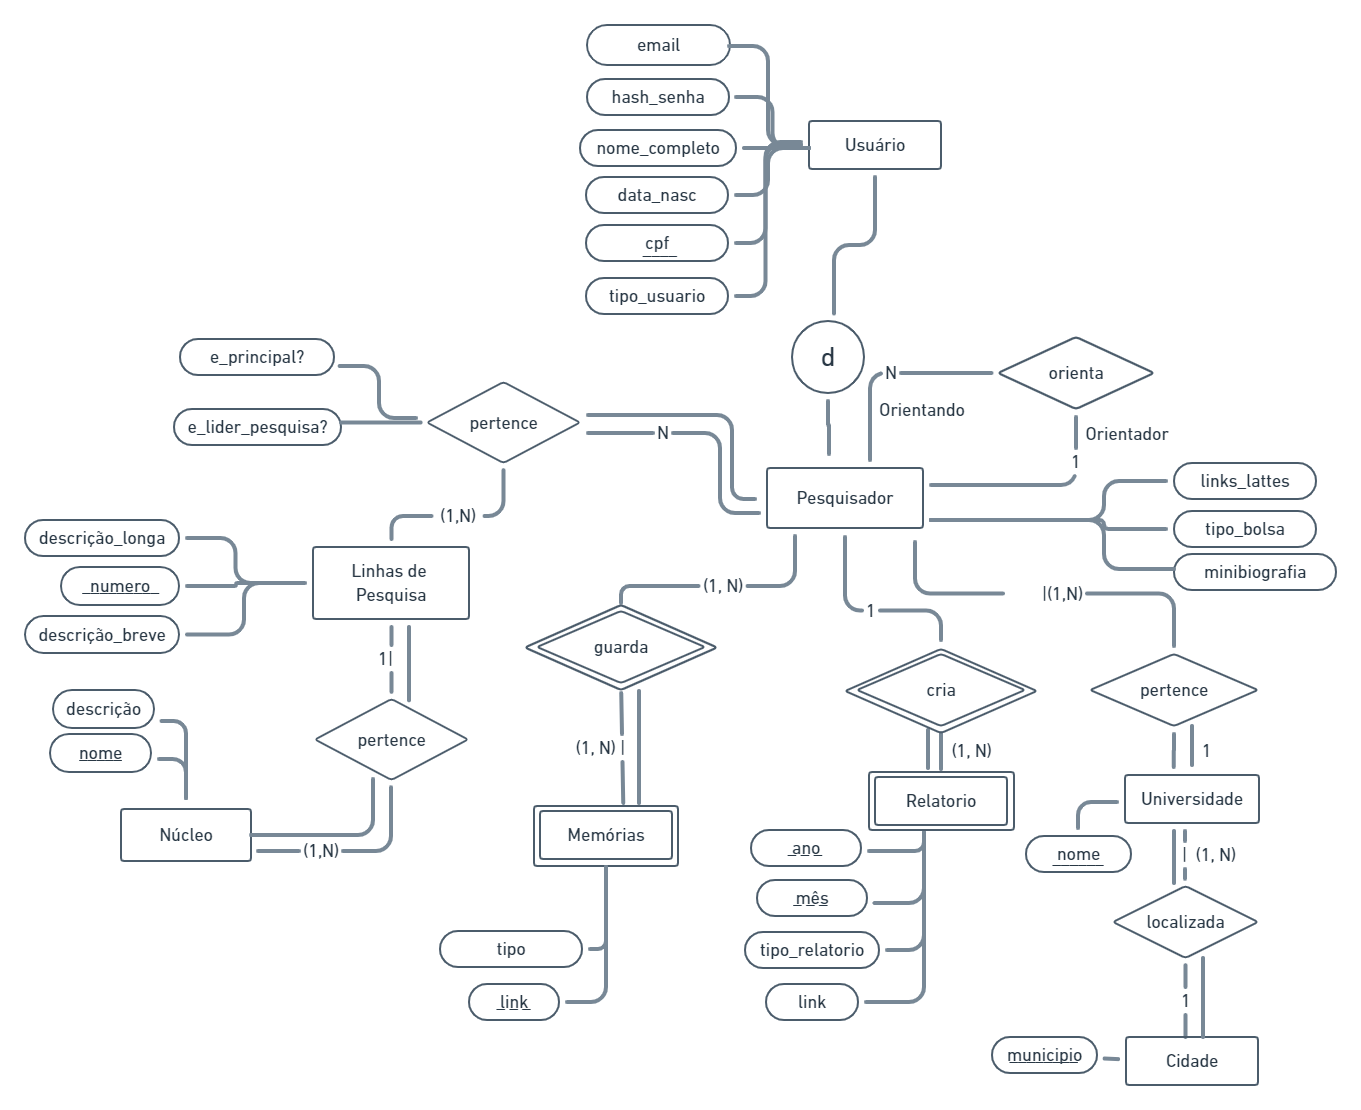
\includegraphics[width=19cm]{figuras/Diagrama.png}
    \caption{Diagrama}
    \label{fig:logolatex}
\end{figure}
\clearpage
\subsection{Tabela de metadados}
Tabelas de metadados com a descrição do tipo
de atributos por tipo-entidade e suas restrições.

\begin{table}[h]
    \centering
    \vspace{0.5cm}
    \begin{tabular}{ |p{2,5cm}|p{3cm}|p{4cm}|p{5,3cm}|  }
        Tipo-Entidade & Atributo                              & Tipo          & Restrições                                       \\ % Note a separação de col. e a quebra de linhas

        \hline
        Linhas \linebreak de Pesquisa
                      &                                       &               &                                                  \\
                      & Descrição curta                       & Monovalorado  & Obrigatório                        \linebreak    \\
                      & Número\underline{ }\underline{ }linha & Identificador & Obrigatório                         \linebreak   \\
                      & Descrição longa                       & Monovalorado  & Opcional, <= 280 caracteres           \linebreak \\
        \hline
    \end{tabular}
    \caption{Tabela de Tipo-Entidade das Linhas de pesquisa.}
\end{table}


\begin{table}[h]
    \centering
    \vspace{0.5cm}
    \begin{tabular}{ |p{2,5cm}|p{3cm}|p{4cm}|p{5,3cm}|  }
        Tipo-Entidade & Atributo         & Tipo          & Restrições                                \\ % Note a separação de col. e a quebra de linhas

        \hline
        Núcleo        &                  &               &                                           \\
                      & Nome             & Identificador & Obrigatório        \linebreak             \\
                      & Descrição Núcleo & Monovalorado  & Obrigatório, <= 400 caracteres \linebreak \\

        \hline
    \end{tabular}
    \caption{Tabela de Tipo-Entidade do Núcleo.}
\end{table}


\begin{table}[h]
    \centering
    \vspace{0.5cm}
    \begin{tabular}{ |p{2,5cm}|p{3cm}|p{4cm}|p{5,3cm}|  }
        Tipo-Entidade & Atributo & Tipo          & Restrições                                \\ % Note a separação de col. e a quebra de linhas

        \hline
        Memórias
                      &          &               &                                           \\
                      & Link     & Chave parcial & Obrigatório    \linebreak                 \\
                      & Tipos    & Monovalorado  & Video \linebreak Imagem \linebreak Artigo \\

        \hline
    \end{tabular}
    \caption{Tipos de atributos por tipo-entidade da Memória.}
\end{table}


\begin{table}[h]
    \centering
    \vspace{0.5cm}
    \begin{tabular}{ p{2,5cm}|p{3cm}|p{4cm}|p{5,3cm}|  }


        Tipo-Entidade & Atributo      & Tipo            & Restrições                                             \\ % Note a separação de col. e a quebra de linhas

        \hline
        % para uma linha horizontal
        Usuario
                      &               &                 &                                                        \\
                      & Cpf           & Identificador   & Obrigatório            \linebreak                      \\
                      & E-mail        & Chave candidata & Obrigatório        \linebreak                          \\
                      & Nome completo & Chave candidata & Obrigatório                        \linebreak          \\
                      & Data nasc     & Monovalorado    & Obrigatório                        \linebreak          \\
                      & Hash Senha    & Monovalorado    & Obrigatório                        \linebreak          \\
                      & Tipo          & Monovalorado    & Administrador\linebreak Pesquisador\linebreak Pescador \\

        \hline
    \end{tabular}
    \caption{Tabela de Tipo-Entidade do Usuario.}
\end{table}

\begin{table}[h]
    \centering
    \vspace{0.5cm}
    \begin{tabular}{ p{2,5cm}|p{3cm}|p{4cm}|p{5,3cm}|  }

        Tipo-Entidade & Atributo      & Tipo            & Restrições                                                     \\ % Note a separação de col. e a quebra de linhas
        \hline
        Pesquisador
                      &               &                 &                                                                \\
                      & Link Lattes   & Chave candidata & Obrigatório                                        \linebreak  \\
                      & Tipo de bolsa & Monovalorado    & Obrigatório                                        \linebreak  \\
                      & Minibiografia & Monovalorado    & Obrigatório, <= 280 caracteres                      \linebreak \\
        \hline
    \end{tabular}
    \caption{Tabela de Tipo-Entidade do Pesquisador.}
\end{table}

\clearpage

\begin{table}[h]
    \centering
    \vspace{0.5cm}
    \begin{tabular}{ p{2,5cm}|p{3cm}|p{4cm}|p{5,3cm}|  }


        Tipo-Entidade & Atributo & Tipo          & Restrições                                                      \\ % Note a separação de col. e a quebra de linhas
        \hline
        Relatório
                      &          &               &                                                                 \\
                      & Mês      & Chave parcial & Obrigatório                                          \linebreak \\
                      & Ano      & Chave parcial & Obrigatório                                          \linebreak \\
                      & Tipo     & Monovalorado  & Mensal\linebreak Trimestral\linebreak Anual                     \\
        \hline
    \end{tabular}
    \caption{Tabela de Tipo-Entidade do Relatório}
\end{table}


\begin{table}[h]
    \centering
    \vspace{0.5cm}
    \begin{tabular}{ p{2,5cm}|p{3cm}|p{4cm}|p{5,3cm}|  }


        Tipo-Entidade & Atributo & Tipo          & Restrições                                                      \\ % Note a separação de col. e a quebra de linhas
        \hline
        Universidade
                      &          &               &                                                                 \\
                      & Nome     & Identificador & Obrigatório                                          \linebreak \\
        \hline
    \end{tabular}
    \caption{Tabela de Tipo-Entidade do Universidade}
\end{table}


\begin{table}[h]
    \centering
    \vspace{0.5cm}
    \begin{tabular}{ p{2,5cm}|p{3cm}|p{4cm}|p{5,3cm}|  }


        Tipo-Entidade & Atributo  & Tipo          & Restrições                                                      \\ % Note a separação de col. e a quebra de linhas
        \hline
        Cidade
                      &           &               &                                                                 \\
                      & Municipio & Identificador & Obrigatório                                          \linebreak \\
        \hline
    \end{tabular}
    \caption{Tabela de Tipo-Entidade da Cidade}
\end{table}

\clearpage

\section{Modelo Relacional}
\subsection{Pesquisador}

pesquisador (\underline{cpf\underline{ }\underline{ }usuário},
tipo\underline{ }\underline{ }bolsa,
minibiografia,
cod\underline{ }\underline{ }orientador)

\begin{itemize}
    \item cpf\underline{ }\underline{ }usuário referencia usuario;
    \item cod\underline{ }\underline{ }orientador referencia o proprio pesquisador;
\end{itemize}

\subsection{Memórias}
memorias (tipo,
\underline{link},
\underline{cpf\underline{ }\underline{ }usuário})

\begin{itemize}
    \item \underline{cpf\underline{ }\underline{ }usuário} referencia pesquisador;
\end{itemize}

\subsection{Relatórios}
memorias (link,
\underline{ano},
\underline{mes},
\underline{link\underline{ }\underline{ }lattes})

\begin{itemize}
    \item \underline{cpf\underline{ }\underline{ }usuário} referencia pesquisador;
\end{itemize}
\subsection{Linhas de Pesquisa}
linhas\underline{ }\underline{ }pesquisa (\underline{numero\underline{ }\underline{ }linha},
decricao\underline{ }\underline{ }curta,
descricao\underline{ }\underline{ }longa,
nome\underline{ }\underline{ }nucleo)


\begin{itemize}
    \item nome\underline{ }\underline{ }nucleo referencia nucleo;
\end{itemize}

%\textcolor{pink}{tyestasasasasasas}
\subsection{Núcleos}
nucleo (\underline{nome}, decricao\underline{ }\underline{ }nucleo)

\subsection{Pertence}
pertence (é\underline{ }\underline{ }principal,
é\underline{ }\underline{ }lider\underline{ }\underline{ }pesquisa,
\underline{cpf\underline{ }\underline{ }usuário},
\underline{numero\underline{ }\underline{ }linha})


\begin{itemize}
    \item link\underline{ }\underline{ }lattes referencia pesquisador;
    \item numero\underline{ }\underline{ }linha referencia Linhas de Pesquisa.
\end{itemize}

\subsection{Usuario}
usuario (\underline{cpf}, email, nome\underline{ }\underline{ }completo, data\underline{ }\underline{ }nasc, hash\underline{ }\underline{ }senha, tipo)

%Qual o identificador do pesquisador, é o CPF do usuario?

\end{document}

